% Define document class
\documentclass[twocolumn,twocolappendix]{aastex701}

\usepackage{graphicx}
\usepackage{xcolor}

% user-defined commands
\newcommand{\todo}[1]{{\color{red}#1}}
\newcommand{\osuaffil}{Department of Astronomy, The Ohio State University, 140 W. 18th Ave, Columbus, OH 43210, USA}
\newcommand{\ccappaffil}{Center for Cosmology and AstroParticle Physics, The Ohio State University, 191 W. Woodruff Ave., Columbus, OH 43210, USA}

\shorttitle{}
\shortauthors{}

\begin{document}

% Title
\title{Chemical Clocks Paper II: Chemical Evolution Models}

% Author list
\author[0000-0003-3781-0747]{Liam O.\ Dubay}
\affiliation{\osuaffil}
\affiliation{\ccappaffil}
\email{dubay.11@osu.edu}
\correspondingauthor{Liam Dubay}
\author{co-authors}
\email{}
\affiliation{}
\shortauthors{Dubay et al.}
% People who commented on this section in the data paper:
% Sofia Feltzing, Alexandre Roman Lopes

\begin{abstract}
    Abstract.
\end{abstract}

\section{Introduction}
\label{sec:introduction}

\section{Data}
\label{sec:data}

\section{Models}
\label{sec:models}

We adopt the same basic setup as the models of \citet{johnson_stellar_2021}. Using the Versatile Integrator for Chemical Evolution \citep[VICE;][]{johnson_impact_2020}, we model the disk as a series of concentric rings with a width of 100 pc, each of which is a separate one-zone GCE model with instantaneous mixing. Stellar populations migrate between zones according to the prescription of \citet{dubay_galactic_2024}, and may enrich the zones they travel through with the products of SN Ia and AGB nucleosynthesis. We adopt a \citet{kroupa_variation_2001} initial mass function (IMF).

% AGB yields
Cerium enrichment in our models proceeds through a prompt, metallicity-independent $r$-process channel, and a delayed, metallicity-dependent $s$-process channel. We assume that massive stars contribute the $r$-process yield. Assuming a Solar $r$-process fraction for Ce of $f_{\rm Ce,\odot}^r=0.23$ \citep{arlandini_neutron_1999}, we assign the CCSN yield of Ce to be
\begin{equation}
    y_{\rm Ce}^{\rm CC} = f_{\rm Ce,\odot}^r (Z_{\rm Ce,\odot} / Z_{\rm Mg,\odot}) y_{\rm Mg}^{\rm CC}.
    \label{eq:rproc-yield}
\end{equation}
This results in a CCSN ``plateau'' of $\bracket[Mg]{Ce}_{\rm CC}=\log_{10}(f_{\rm Ce,\odot}^r) \approx -0.64$, akin to the low-Ia $\bracket[Fe]{\alpha}$ plateau. We have also explored a delayed neutron star merger channel for $r$-process enrichment, but due to the low Solar $r$-process fraction of Ce, it has a small effect on our models.

\begin{figure*}
    \centering
    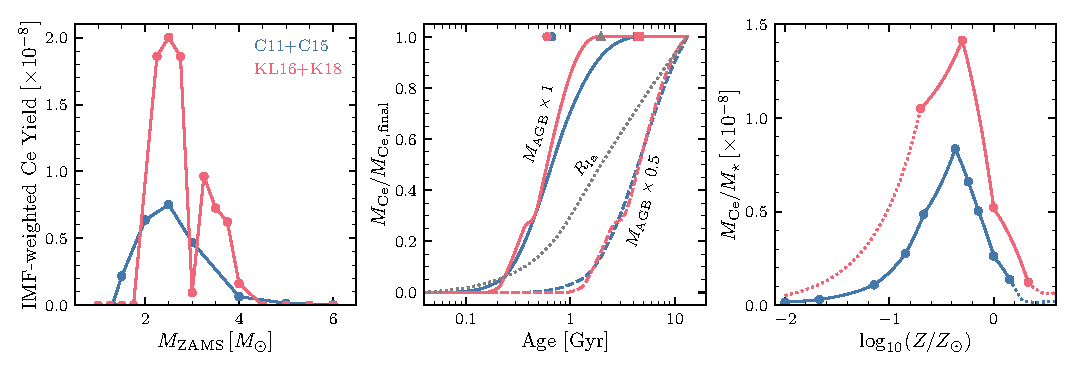
\includegraphics[width=\textwidth]{figures/ssp_yields.pdf}
    \caption{{\it Left:} The IMF-weighted Ce mass yield from AGB stars as a function of ZAMS mass at Solar metallicity. {\it Center:} The net mass of Ce produced by AGB stars over time from a single stellar population at Solar metallicity. The $y$-axis is normalized to the value at $t=13.2\Gyr$. The solid curves represent the un-altered yields, the dashed curves plot the mass-scaled yields with $M_{\rm AGB}\times0.5$, and the dotted gray curve plots the cumulative SN Ia enrichment curve for reference. The points along the top axis indicate the ages at which 50\% of the total mass has been produced by the un-altered yields (circles), SN Ia yield (triangle), and mass-scaled yields (squares). {\it Right:} The mass of Ce produced by a $13.2\Gyr$ old stellar population as a function of metallicity normalized by the initial mass. The points mark values of the metallicity grid for each study, the solid lines represent linear interpolation between each grid value, and the dotted lines represent a linear extrapolation beyond the grid boundaries.}
    \label{fig:ssp-yields}
\end{figure*}

For AGB stars, we explore two sets of yield grids: those of \citet[][hereafter C11+C15]{cristallo_evolution_2011,cristallo_evolution_2015}, and those of \citet{karakas_stellar_2016} and \citet[][hereafter KL16+K18]{karakas_heavy-element_2018}. \todo{Briefly cover the differences between them}. The KL16+K18 grid only extends down to $\bracket{M}\approx-0.7$, so we linearly extrapolate the yield below this point, assuming a yield of 0 for a zero-metallicity star. Figure \ref{fig:ssp-yields} shows the dependence of the Ce yield on mass and metallicity. For both yield sets, most Ce is produced by $2-3\Msun$ AGB stars, resulting in a median enrichment timescale of $\sim600\Myr$. The yield also peaks at $\bracket{M}\approx-0.4$ and declines sharply above Solar metallicity for both sets, although the KL16+K18 yields produce more Ce overall by roughly a factor of 2.

% CCSN yields
In order for our models to reach a consistent value of [Ce/Mg], we adopt a different CCSN yield scale for each AGB yield set. 
\citet{weinberg_scale_2024} used a measurement of the mean Fe yield of CCSNe by \citet{rodriguez_iron_2023} to calibrate an empirical scale for CCSN yields. They found that the population-averaged yield of Mg is approximately equal to the Solar abundance, in other words $y_{\rm Mg}^{\rm CC}/Z_{\rm Mg,\odot}\approx1$. In comparison, theoretical yield predictions typically range over $y^{\rm CC}/Z_\odot\approx2-3$. We find that in order for our models to reach super-Solar [Ce/Mg] by the present day, we require $y^{\rm CC}/Z_\odot=1$ for the C11+C15 yields and $y^{\rm CC}/Z_\odot=1$ for the KL16+K18 yields. \citet{johnson_milky_2025} discuss the consequences of the CCSN yield scale on the chemical evolution of the Milky Way disk. We adopt the Solar abundances of \citet{asplund_chemical_2009}, and we adopt $y_{\rm Mg}^{\rm CC}=7.06\times10^{-4}$ for $y/Z_\odot=1$ and $y_{\rm Mg}^{\rm CC}=1.41\times10^{-3}$ for $y/Z_\odot=2$.
% We adopt the empirical yields of \citet{weinberg_scale_2024} for CCSN and SN Ia nucleosynthesis. These yields are scaled to the mean Fe yield of CCSNe measured by \citet{rodriguez_iron_2023} and assume a CCSN plateau of $\bracket[Fe]{Mg}=+0.45$ to set the Mg yield. The population-averaged SN Ia yield of Fe is
% \begin{equation}
%     y_{\rm Fe}^{\rm Ia} = R_{\rm Ia} \bar m_{\rm Fe}^{\rm Ia} = 9.1\times10^{-4},
% \end{equation}
% assuming a time-integrated SN Ia rate of $R_{\rm Ia}=\SI{1.3e-3}{\per\Msun}$ \citep{maoz_star_2017} and a mean Fe yield per SN Ia of $\bar m_{\rm Fe}^{\rm Ia}=0.7\Msun$ \citep{howell_effect_2009}. These yields are a factor of $\sim2-3$ lower than theoretical predictions, but can still reproduce present-day gas abundances by appropriately scaling the outflows \citep[e.g.,][]{johnson_milky_2025}. For the SN Ia delay-time distribution, we adopt the ``plateau DTD'' of \citet{dubay_galactic_2024}, which reproduces the low-Ia sequence more closely than a $t^{-1}$ power-law.

We use a prescription for mass-loaded outflows to reproduce the present-day gas metallicity as a function of radius. We implement an exponential prescription for the outflow mass-loading factor:
\begin{equation}
    \eta \equiv \frac{\dot\Sigma_{\rm gas}}{\dot\Sigma_\star} = \eta_\odot \exp\Big(\frac{R_{\rm gal}-R_\odot}{R_\eta}\Big),
\end{equation}
where we adopt $\eta_\odot=0.4$ and $R_\eta=5\kpc$ to reproduce a radial metallicity gradient of $-0.06\dex\kpc^{-1}$ \citep{mendez-delgado_gradients_2022}. This is a practical choice to reproduce stellar abundances across the Milky Way disk with few additional parameters. \citet{johnson_milky_2025} discuss the mass-loaded outflows in disk galaxies. Similar results can also be achieved using radial gas flows, but their implementation in GCE models is less straightforward \citep{johnson_constraints_2025}.

For our fiducial model, we adopt the ``inside-out'' star formation history from \citet{johnson_stellar_2021}. This SFH can reproduce the stellar age--metallicity and age--[$\alpha$/Fe] relations across the disk from \citet{feuillet_spatial_2019}, although it does not reproduce the Milky Way's $\alpha$-bimodality \citep{johnson_stellar_2021}. Our primary goal is to explain the Ce abundance patterns in high-Ia stars, but the lack of a distinct low-Ia population is a limitation of our models. Star formation proceeds according to a \citet{schmidt_rate_1959} law $\dot\Sigma_\star\propto\Sigma_g^k$ with $k=1.5$ \citep{kennicutt_global_1998}, with the detailed implementation described by \citet{johnson_milky_2025}. The star formation rate in each zone is normalized to reproduce the double-exponential radial stellar density profile of \citet{bland-hawthorn_galaxy_2016}.

\section{Results}
\label{sec:results}

\begin{figure}
    \centering
    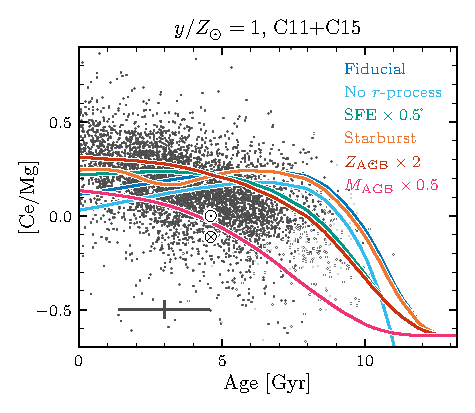
\includegraphics[width=\linewidth]{figures/model_comparison.pdf}
    \caption{Comparison of [Ce/Mg]--age trends predicted by multi-zone models. The blue curve represents the gas abundance evolution in fiducial model, and all other curves represent models that differ by one parameter. All models adopt the $y/Z_\odot=1$ CCSN yield scale and the C11+C15 AGB yields. The gray filled (open) points represent low-Ia (high-Ia) stars in the Solar neighborhood ($7\leq R_g<9\kpc$, $z_{\rm max}<0.5\kpc$) with $-0.1\leq\bracket{Mg}<+0.1$. The gray error bars indicate the median uncertainties for the plotted sample, the $\odot$ symbol marks the Solar age and [Ce/Mg] value, and the $\otimes$ symbol represents the Solar $s$-process fraction \citep{arlandini_neutron_1999}.}
    \label{fig:model-comparison}
\end{figure}

Figure \ref{fig:model-comparison} compares the predicted [Ce/Mg]--age relation from our models against observed trends for Solar-metallicity stars in the Solar neighborhood. These models all adopt the $y/Z_\odot=1$ and C11+C15 yields, but the models at the higher yield scale show similar trends. The fiducial model starts at the CCSN plateau of $\bracket[Mg]{Ce}_{\rm CC}\approx -0.64$ and rises steadily to a maximum of $\bracket[Mg]{Ce}\approx+0.2$ at a lookback time of 7 Gyr, then slowly declines by $\sim0.1\dex$ to the present day. The model completely fails to reproduce the trend observed in the data, over-predicting [Ce/Mg] for the oldest stars and under-predicting for the youngest. The fiducial model also fails to reproduce the Solar [Ce/Mg] at the age of the Sun, which could be fixed by scaling down the AGB yield by $\sim30\%$, although this would worsen the under-prediction for the youngest stars. 
% \todo{This may not be as big of a problem if the Sun was born at a smaller radius, where [Ce/Mg] ratios are lower.}

In theory, an $r$-process channel with long delay times could increase [Ce/Mg] over time. However, Figure \ref{fig:model-comparison} illustrates that the $r$-process contribution is small, $\sim0.1\dex$, over most of the model's evolution. The Solar $r/s$ ratio would need to be much higher than expected in order for a delayed $r$-process channel to have a significant effect at late times.

We explore two modifications to the star formation history in Figure \ref{fig:model-comparison}. First, we reduce the star formation efficiency (SFE) by half (i.e., doubling $\tau_\star$), which leads to a more gradual increase in [Ce/Mg] over time \todo{(why?)}. This alleviates the over-prediction problem for old stars, but results in a [Ce/Mg]--age relation that is flat, not increasing, over the past $5\Gyr$. Reducing the SFE also worsens agreement with the data for other observables, such as the [Fe/Mg]--[Mg/H] and age--metallicity relations. Second, we add a recent starburst described by a Gaussian in time:
\begin{equation}
    \dot\Sigma_{\rm \star, burst}(t) = \dot\Sigma_{\rm \star,fiducial}(t) \Big(1 + A_b e^{-(t-t_b)^2/2\sigma^2_b}\Big),
\end{equation}
where $A_b=2$ is the amplitude of the starburst, $t_b=10.2\Gyr$ is the time of the local maximum star formation rate, and $\sigma_b=1\Gyr$ is the width of the Gaussian. We find that such a starburst leads to an increase in [Ce/Mg] over $\sim2\Gyr$, but the trend is not long-term.

We next investigate modifications to the metallicity and mass dependence of the AGB yields. Figure \ref{fig:ssp-yields} shows that the Ce yield falls off dramatically above Solar metallicity. By scaling up the metallicity for a given yield (effectively shifting the distribution to higher $Z$), Solar-metallicity AGB stars can produce a greater mass of Ce. Figure \ref{fig:model-comparison} shows the result for a model with AGB metallicities scaled by a factor of 2 ($Z_{\rm AGB}\times2$). [Ce/Mg] increases slower, as the yield at low metallicities is reduced, while at later times the [Ce/Mg] surprasses that of the fiducial model. The metallicity scaling is effective in the Solar neighborhood, but detrimental to the [Ce/Mg] ratios in the outer galaxy, where the gas metallicity is too low.

Figure \ref{fig:ssp-yields} shows that AGB stars below $2\Msun$ contribute very little Ce. As a result, the median enrichment time (i.e., the time after star formation at which 50\% of the total Ce mass has been produced) for both yield sets is only $\sim600\Myr$, whereas the Milky Way data show increasing [Ce/Mg] over the past $\sim6\Gyr$. We therefore explore another modification to the yields where we scale the ZAMS mass of an AGB star corresponding to a given yield by a factor of 0.5 (i.e., a $1\Msun$ star now contributes the mass of Ce that would be produced by a $2\Msun$ star in the fiducial prescription). Figure \ref{fig:model-comparison} shows that a model with these mass-scaled yields evolves much slower than our other models. Notably, this model predicts monotonically increasing [Ce/Mg] up to the present day, and closely reproduces the Solar abundance at the Solar age. This model does under-predict the median trend by $\sim0.2\dex$, which could be corrected by amplifying the total Ce yield.

\begin{figure}
    \centering
    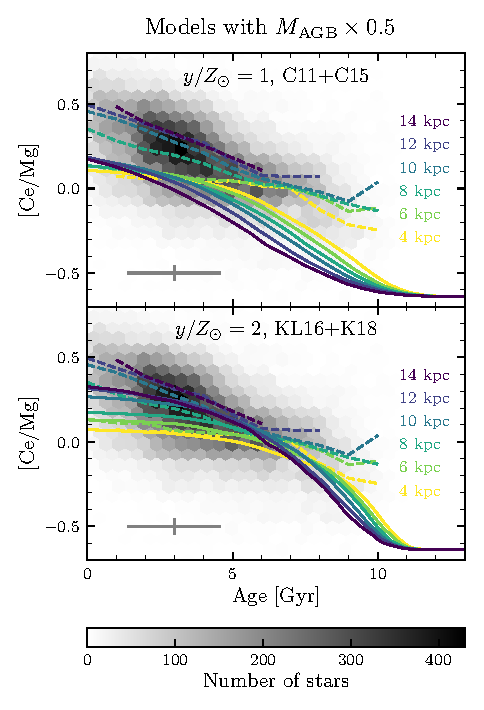
\includegraphics[width=\linewidth]{figures/model_radius_trends.pdf}
    \caption{The evolution of [Ce/Mg] predicted by multi-zone models with mass-scaled AGB yields. The solid curves plot the model predictions for six different zones, color-coded by radius. The dashed curves plot the median [Ce/Mg] in bins of stellar age for the MWM sample with $z_{\rm max}<0.5\kpc$ at each radius. The 2-D histogram indicates the global distribution of MWM stars, and the error bars indicate the median age and abundance errors for the sample.}
    \label{fig:model-radius-trends}
\end{figure}

We showed in Section \ref{sec:residual-abundances} that the [Ce/Mg]--age relation varies significantly across the Galaxy, and a GCE model that explains the $[s/\alpha]$ ratios in the Milky Way needs to explain this variation. Figure \ref{fig:model-radius-trends} plots the gas abundance evolution at different radii for two of our models with mass-scaled AGB yields. The scale of CCSN yields has a large effect on the [Ce/Mg] abundance evolution\textemdash models with higher yields reach the equilibrium abundance faster \citep[see][]{johnson_milky_2025}. While the model with $y/Z_\odot=1$ and C11+C15 yields reproduces the overall [Ce/Mg]--age trend, it predicts that the [Ce/Mg] in the inner Galaxy is {\it higher} than in the outer Galaxy at the same age, a qualitatively different trend than shown by the data. This discrepancy is resolved in the higher-yield model, which predicts similar abundance evolution at all radii for ages $>8\Gyr$ and increasing [Ce/Mg] with radius for ages $<8\Gyr$. This model is not perfect\textemdash the present-day radial [Ce/Mg] gradient is too shallow\textemdash but it predicts qualitatively similar trends between [Ce/Mg], age, and radius to the data.

\begin{figure*}
    \centering
    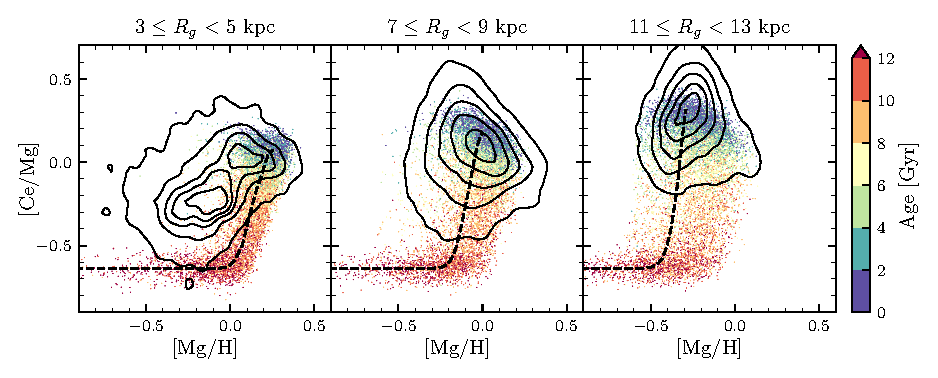
\includegraphics[width=\linewidth]{figures/model_cemg_mgh.pdf}
    \caption{Stellar abundance distributions in three different radial bins predicted by the model with $y/Z_\odot=2$, KL16+K18, and $M_{\rm AGB}\times0.5$. Stars in each panel are restricted to $z_{\rm max}<2\kpc$. Each point represents a model stellar population, color-coded by age. A Gaussian scatter has been applied to each model stellar population based on the median abundance and age errors in the MWM sample. For visual clarity, only a random sample of 10,000 points is plotted in each panel. The dashed curve plots the gas abundance track at the mean radius in each bin. The solid contours show the 10th, 30th, 50th, 70th, and 90th percentiles of the MWM data in each region.}
    \label{fig:model-cemg-mgh}
\end{figure*}

Figure \ref{fig:model-cemg-mgh} shows the [Ce/Mg]--[Mg/H] relation predicted by the best model in three different radial bins. In the Solar neighborhood and outer Galaxy, the model stellar populations overlap the highest-density region of the data, and the model qualitatively reproduces the stellar age relation seen in Figure \ref{fig:cemg-mgh-age}. The region with the highest [Ce/Mg] is not reproduced by the model, which could be attributed to underestimated uncertainties for the MWM [Ce/H] abundances,  The model is less successful in the inner Galaxy, where it completely misses the low-Ia sequence. Due to the long AGB enrichment timescale combined with the high star formation rate, the [Ce/Mg] ratio only increases from the $r$-process plateau above $\bracket{Mg}>0$. While not shown in Figure \ref{fig:model-cemg-mgh}, the problem is even worse for the halo population, which exhibits Solar [Ce/Mg] ratios at $\bracket{Mg}\sim-1$ (see Section \ref{sec:halo}).

\todo{Discuss possible ``blue straggler'' model in a sub-section.}

In summary, chemical evolution models with standard AGB yield prescriptions fail to reproduce the negative [Ce/Mg]--age trend observed in the Milky Way's high-Ia disk. By shifting the yield distribution to lower-mass AGB stars, we successfully reproduced the qualitative [Ce/Mg]--age--radius relation of the high-Ia disk. However, this model under-predicts the [Ce/Mg] ratios of the low-Ia and halo populations, suggesting that some prompt Ce enrichment beyond the $r$-process contribution is needed.

\section{Conclusions}
\label{sec:conclusions}

\begin{itemize}
    \item A chemical evolution model of the disk is unable to reproduce the [Ce/Mg]--age relation with standard AGB yield prescriptions. After shifting the production of Ce to lower-mass AGB stars to increase the enrichment timescale, our model qualitatively reproduces the [Ce/Mg]--age trends across the high-Ia disk. However, our model fails to reproduce the abundances of low-Ia and halo stars, so more work is needed to understand the chemical evolution of the $s$-process.
\end{itemize}

\section*{Acknowledgements}

% From the Center for Belonging and Social Change, https://cbsc.osu.edu/about-us/land-acknowledgement
We would like to acknowledge the land that The Ohio State University occupies is the ancestral and contemporary territory of the Shawnee, Potawatomi, Delaware, Miami, Peoria, Seneca, Wyandotte, Ojibwe and many other Indigenous peoples. Specifically, the university resides on land ceded in the 1795 Treaty of Greeneville and the forced removal of tribes through the Indian Removal Act of 1830. As a land grant institution, we want to honor the resiliency of these tribal nations and recognize the historical contexts that has and continues to affect the Indigenous peoples of this land.

\software{}

\appendix

\section{Reproducibility}
\label{app:reproducibility}

\bibliography{references}
\bibliographystyle{aasjournalv7}

\end{document}
